\section{Worked Examples}

\bigskip

\subsection{Gradient Descent}
\label{worked-gradient-descent}

\medskip

\begin{enumerate}
    \setlength{\itemsep}{1em}
    \item Initialize: Let the weights be $\theta_1 = 0.5$ and $\theta_2 = 1.0$. Use a learning rate $\alpha = 0.01$.
    \item Dataset: Consider three data points $(x_{i1}, x_{i2}, y_i)$:
    \begin{itemize}
        \item Point 1: $(1, 2, 5)$
        \item Point 2: $(2, 1, 4)$
        \item Point 3: $(0, 3, 7)$
    \end{itemize}
    \item Define Model and Loss: The prediction is $\hat{y}_i = \theta_1 x_{i1} + \theta_2 x_{i2}$. We use Mean Squared Error:
    $$L(\theta) = \frac{1}{3} \sum_{i=1}^3 (\theta_1 x_{i1} + \theta_2 x_{i2} - y_i)^2$$
    \item Calculate Predictions:
    \begin{itemize}
        \item $\hat{y}_1 = (0.5)(1) + (1.0)(2) = 2.5$
        \item $\hat{y}_2 = (0.5)(2) + (1.0)(1) = 2.0$
        \item $\hat{y}_3 = (0.5)(0) + (1.0)(3) = 3.0$
    \end{itemize}
    \item Compute Gradients: The partial derivative for each weight $\theta_j$ is:
    $$\frac{\partial L}{\partial \theta_j} = \frac{2}{3} \sum_{i=1}^3 (\hat{y}_i - y_i)x_{ij}$$
    For $\theta_1$:
    $$\frac{\partial L}{\partial \theta_1} = \frac{2}{3} [(2.5-5)(1) + (2.0-4)(2) + (3.0-7)(0)] = \frac{2}{3} [-2.5 - 4 + 0] = -4.33$$
    For $\theta_2$:
    $$\frac{\partial L}{\partial \theta_2} = \frac{2}{3} [(2.5-5)(2) + (2.0-4)(1) + (3.0-7)(3)] = \frac{2}{3} [-5 - 2 - 12] = -12.67$$
    \item Update Weights:
    $$\theta_{new} = \theta_{old} - \alpha \frac{\partial L}{\partial \theta}$$
    $$\theta_1 = 0.5 - (0.01 \times -4.33) = 0.5433$$
    $$\theta_2 = 1.0 - (0.01 \times -12.67) = 1.1267$$
\end{enumerate}


\newpage

\subsection{Gradient Descent (Matrix Form)}

\begin{enumerate}
    \setlength{\itemsep}{1em}
    \item Initialize: Define the weight vector $\theta$, feature matrix $X$, and target vector $y$:
    $$\theta = \begin{bmatrix} 0.5 \\ 1.0 \end{bmatrix}, \quad X = \begin{bmatrix} 1 & 2 \\ 2 & 1 \\ 0 & 3 \end{bmatrix}, \quad y = \begin{bmatrix} 5 \\ 4 \\ 7 \end{bmatrix}$$
    
    \item Define Model and Loss:
    The predictions are $\hat{y} = X\theta$, and the Mean Squared Error is:
    $$L(\theta) = \frac{1}{3} \|X\theta - y\|^2$$

    \item Calculate Predictions:
    $$\hat{y} = \begin{bmatrix} 1 & 2 \\ 2 & 1 \\ 0 & 3 \end{bmatrix} \begin{bmatrix} 0.5 \\ 1.0 \end{bmatrix} = \begin{bmatrix} (1)(0.5) + (2)(1.0) \\ (2)(0.5) + (1)(1.0) \\ (0)(0.5) + (3)(1.0) \end{bmatrix} = \begin{bmatrix} 2.5 \\ 2.0 \\ 3.0 \end{bmatrix}$$

    \item Compute Gradient:
    The gradient vector $\nabla L(\theta)$ is calculated as:
    $$\nabla L(\theta) = \frac{2}{3} X^T (\hat{y} - y)$$
    First, find the error vector $(\hat{y} - y)$:
    $$\hat{y} - y = \begin{bmatrix} 2.5 - 5 \\ 2.0 - 4 \\ 3.0 - 7 \end{bmatrix} = \begin{bmatrix} -2.5 \\ -2.0 \\ -4.0 \end{bmatrix}$$
    Then, multiply by the transposed feature matrix $X^T$:
    $$\nabla L(\theta) = \frac{2}{3} \begin{bmatrix} 1 & 2 & 0 \\ 2 & 1 & 3 \end{bmatrix} \begin{bmatrix} -2.5 \\ -2.0 \\ -4.0 \end{bmatrix} = \frac{2}{3} \begin{bmatrix} -6.5 \\ -19.0 \end{bmatrix} = \begin{bmatrix} -4.33 \\ -12.67 \end{bmatrix}$$

    \item Update Weights:
    Using learning rate $\alpha = 0.01$:
    $$\theta_{new} = \theta_{old} - \alpha \nabla L(\theta)$$
    $$\theta_{new} = \begin{bmatrix} 0.5 \\ 1.0 \end{bmatrix} - 0.01 \begin{bmatrix} -4.33 \\ -12.67 \end{bmatrix} = \begin{bmatrix} 0.5433 \\ 1.1267 \end{bmatrix}$$
\end{enumerate}


\newpage

\subsection{XOR Neural Net with ReLU}
\label{worked-XOR-relu-model}

\medskip

Recall the XOR dataset:

\begin{center}
\noindent
\begin{minipage}{0.3\textwidth}
$
X =
\begin{bmatrix}
0 & 0 \\
0 & 1 \\
1 & 0 \\
1 & 1
\end{bmatrix},
\qquad
y =
\begin{bmatrix}
0 \\
1 \\
1 \\
0
\end{bmatrix}
$
\end{minipage}
\begin{minipage}{0.36\textwidth}
\centering
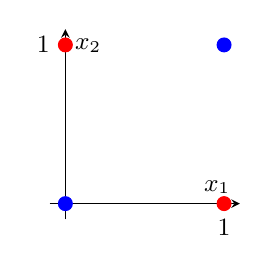
\begin{tikzpicture}
\begin{axis}[
    width=4cm,
    height=4cm,
    xmin=-0.1, xmax=1.1,
    ymin=-0.1, ymax=1.1,
    axis lines=middle,
    xtick={0,1},
    ytick={0,1},
    xlabel={$x_1$},
    ylabel={$x_2$},
    tick label style={font=\small},
    label style={font=\small},
    enlargelimits=false,
    clip=false
]

% Class 0 (blue)
\addplot[
    only marks,
    mark=*,
    mark size=2.5pt,
    blue
]
coordinates {(0,0) (1,1)};

% Class 1 (red)
\addplot[
    only marks,
    mark=*,
    mark size=2.5pt,
    red
]
coordinates {(0,1) (1,0)};

\end{axis}
\end{tikzpicture}
\end{minipage}
\end{center}

A single linear layer has the form
\[
\hat y = w_1 x_1 + w_2 x_2 + b,
\]
which defines a single separating line in $\mathbb{R}^2$.  
XOR is not linearly separable, so no choice of $(w_1,w_2,b)$ can fit all four points.

\bigskip

\textbf{Two–layer ReLU model.}

We now introduce two hidden units with ReLU activation:
\[
\mathrm{ReLU}(z) = \max(0,z).
\]

The network is

\[
\begin{aligned}
z_1 &= w_{11} x_1 + w_{21} x_2 + c_1, \\
z_2 &= w_{12} x_1 + w_{22} x_2 + c_2, \\
h_1 &= \mathrm{ReLU}(z_1), \\
h_2 &= \mathrm{ReLU}(z_2), \\
\hat y &= \alpha h_1 + \beta h_2 + c_3.
\end{aligned}
\]

Choose the parameters (as in the slide):

\[
w_{ij}=1,
\quad
c_1 = 0,
\quad
c_2 = -1,
\quad
(\alpha,\beta) = (1,-2),
\quad
c_3 = 0.
\]

Then

\[
z_1 = x_1 + x_2,
\qquad
z_2 = x_1 + x_2 - 1.
\]

Now evaluate all four inputs.

\[
\begin{array}{c|cccc}
(x_1,x_2) 
& (0,0) & (0,1) & (1,0) & (1,1) \\ \hline
z_1 = x_1+x_2 
& 0 & 1 & 1 & 2 \\[4pt]
z_2 = x_1+x_2-1 
& -1 & 0 & 0 & 1 \\[4pt]
h_1 = \mathrm{ReLU}(z_1) 
& 0 & 1 & 1 & 2 \\[4pt]
h_2 = \mathrm{ReLU}(z_2) 
& 0 & 0 & 0 & 1 \\[4pt]
\hat y = h_1 - 2h_2 
& 0 & 1 & 1 & 0
\end{array}
\]

\bigskip

Thus the network reproduces XOR exactly:
\[
\hat y = y
\quad\text{for all training points.}
\]

\bigskip

\textbf{Why this works.}

Let $s = x_1 + x_2$.  
The hidden layer computes
\[
h_1 = \mathrm{ReLU}(s),
\qquad
h_2 = \mathrm{ReLU}(s-1).
\]

In the diagram below, the dashed line is $s=0$, the solid line is $s=1$, and the shaded band is the region $0 < s \le 1$.  

These two lines partition the plane into three regions:
\[
\quad s \le 0, \quad 0 < s \le 1 \quad s > 1.
\]

\medskip

\noindent
\begin{minipage}[t]{0.55\textwidth}
\vspace{0pt}
\centering
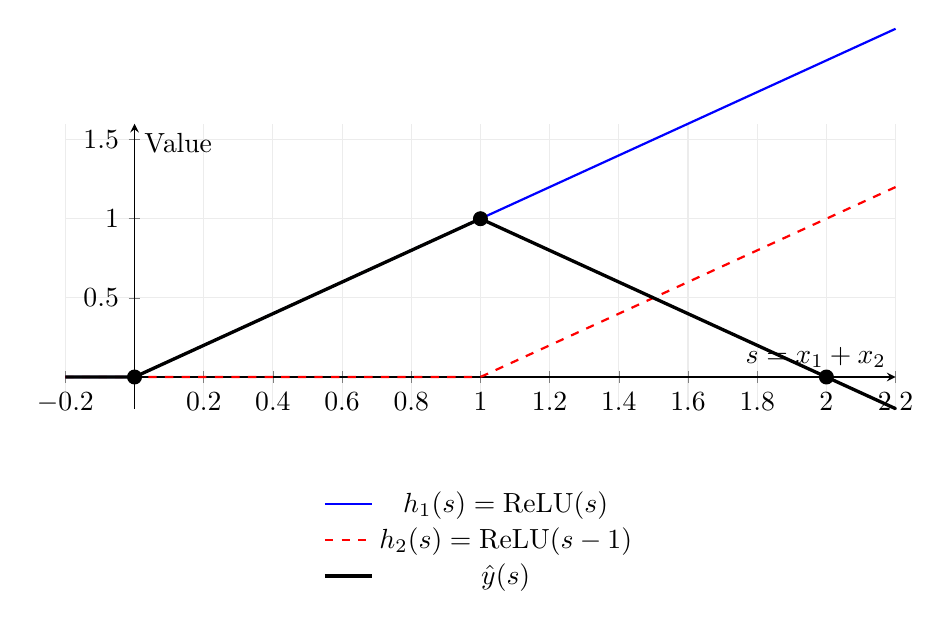
\begin{tikzpicture}
\begin{axis}[
    width=\linewidth,
    height=5.2cm,
    xmin=-0.2, xmax=2.2,
    ymin=-0.2, ymax=1.6,
    axis lines=middle,
    xlabel={$s = x_1 + x_2$},
    ylabel={Value},
    domain=-0.2:2.2,
    samples=300,
    grid=both,
    grid style={gray!15},
    legend style={
        at={(0.5,-0.25)},
        anchor=north,
        draw=none
    },
    clip=false
]

% h1
\addplot[thick, blue]
{max(x,0)};
\addlegendentry{$h_1(s)=\mathrm{ReLU}(s)$}

% h2
\addplot[thick, red, dashed]
{max(x-1,0)};
\addlegendentry{$h_2(s)=\mathrm{ReLU}(s-1)$}

% y
\addplot[very thick, black]
{max(x,0) - 2*max(x-1,0)};
\addlegendentry{$\hat y(s)$}

% XOR points
\addplot[
    only marks,
    mark=*,
    mark size=2.5pt,
    black
]
coordinates {(0,0) (1,1) (2,0)};

\end{axis}
\end{tikzpicture}
\end{minipage}
\hspace{1em}
\begin{minipage}[t]{0.4\textwidth}
\vspace{0pt}

\[
\hat y = h_1 - 2h_2
= \mathrm{ReLU}(s) - 2\,\mathrm{ReLU}(s-1).
\]

\[
\begin{array}{c|c|c|c}
\text{Region} & h_1 & h_2 & \hat y \\ \hline
s \le 0 & 0 & 0 & 0 \\
0 < s \le 1 & s & 0 & s \\
s > 1 & s & s-1 & s - 2(s-1)
\end{array}
\]

\vspace{1em}

On the dataset, $s \in \{0,1,2\}$, so:
\[
\hat y =
\begin{cases}
0 & s=0,\\
1 & s=1,\\
0 & s=2.
\end{cases}
\]

\end{minipage}

\bigskip

The blue curve $h_1(s)=\mathrm{ReLU}(s)$ begins increasing at $s=0$.  
The red dashed curve $h_2(s)=\mathrm{ReLU}(s-1)$ stays flat until $s=1$, then turns on.

The output
\[
\hat y(s)=h_1(s)-2h_2(s)
\]
is the black curve. It rises linearly from $0$ to $1$ as $s$ moves from $0$ to $1$.  
At $s=1$, the second ReLU activates. From that point on, we subtract twice as much as we add, and the function bends downward.

The three dataset values $s=0,1,2$ land exactly at the vertices of this piecewise linear peak, giving outputs $0,1,0$.

\medskip

What matters is the kink at $s=1$.  
A single linear function cannot rise and then turn back down.  
Adding a second ReLU introduces that bend, and that bend is what makes XOR possible.

